\documentclass[12pt,largemargins]{article}
\title{Test 1 Study Guide}
\normalsize
\usepackage{graphicx}
\usepackage{makecell}
\usepackage{enumitem}
\usepackage{multirow}
\usepackage{amsmath}
\usepackage{listings}
\begin{document}
\maketitle

\begin{itemize}
\item[Direct Mapping] 
Consider a machine with a byte addressable main memory of 2 24 bytes and a block size of 32
bytes. Assume that a direct mapped cache consisting of 64 lines is used with this machine. How
is a 24-bit memory address divided into tag, line/set, and word/offset?
How many total bytes of memory can be stored in the cache?
Suppose the byte with address (1101 1011 0100 1110 1010 0111) 2 is stored in the cache. A
number of other bytes are stored with this byte on the same line of cache. What is the highest
address number in this group?
\item[Solution]
Block size = 32 bytes\\
Size of Block/Word = $\log_2 32 = 5$ bytes\\
64 lines $\rightarrow \log_2 64 = 6bytes$\\
\# of lines = $\frac{Cache size}{Block Size} \rightarrow 64 = \frac{Cache Size}{32 bytes}$\\
$\rightarrow 64 * 32 bytes = Cache Size = 2KBytes$\\
Memory block = $24 = tag + 6bytes line/set + 5 word/offset$\\
$\rightarrow 24 - (6+5) = 13bytes = tag$\\
Dividing 110110110100111010100111\\
\begin{tabular}{|c|c|c|}
\hline
13Byte Tag & 6Bytes Word & 5 Bytes word\\
\hline
1101101101001&110101&00111\\
\hline
\end{tabular}\\
The highest addressable is $2^{block size} = 2^{32}$\\
\newpage
\item[Booths Method]
AKA multiplying Two's Compliment Binary Numbers
If at first you don't get the same numbers switch the two numbers\\
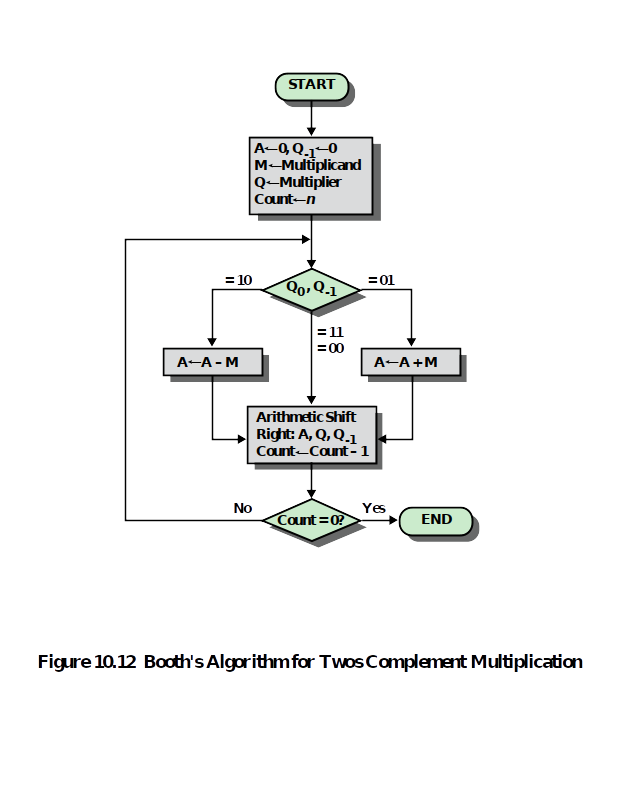
\includegraphics[scale=.8]{booths_method}\\
\item[Instructions Per Seconds]
Assume the following instruction mix for a given benchmark program: 15% stores, 25% loads,
35% branches, and 5% integer addition, and 20% integer multiply. Given a program with 1
million instructions and that load instructions require two cycles, branches require 4 cycles, integer addition and store instructions require 8 cycles and integer multiplies require 16 cycles, compute the overall cycles-per-instruction or CPI.
Determine the Millions of Instructions per Second (MIPS) rate for a 3200-MHz processor.
What is the execution time for this program?
\item[Solution]
$CPI=\sum_{i=1}^{n} \frac{CPI_i x I_i}{I_c}$\\
Instruction Percentage * Inscrution \# Cycles\\
$=.15*8+.25*2+.35*4+.05*8+.2*16=6.7$ cycles per second\\
$MIPS=\frac{Frequency}{CPI*10^6}\rightarrow \frac{3200*10^6}{6.7*10^6} = \frac{3200}{6.7}$ \\
$=4.77.16$ Million Instructions Per Second\\
Total Execution Time $=I_c  *CPI * \frac{1}{F}$\\
$10^6 * 6.7 * \frac{1}{3200*10^6}$\\
$=2.1ms$\\
\item[Sum of Products Stuff]
\begin{tabular}{|c|c|c|c|c|}
\hline
A&B&C&F&SOP\\
\hline
0&0&0&0&0\\
0&0&1&0&0\\
0&1&0&1&$\overline{A}B\overline{C}$\\
0&1&1&1&$\overline{A}BC$\\
1&0&0&1&$A\overline{B}* \overline{C}$\\
1&0&1&1&$A\overline{B}C$\\
1&1&0&0&0\\
1&1&1&0&0\\
\hline
\end{tabular}\\
SOP = $\overline{A}B\overline{C} + \overline{A}BC + A\overline{B}*\overline{C} + A\overline{B}C$\\
POS = $(A+B+C)+(A+B+\overline{C}) + (A+\overline{B}+C)+(A+\overline{B}+\overline{C}) + (\overline{A}+B+C)+(\overline{A}+B+\overline{C})+(\overline{A}+\overline{B}+C)+(\overline{A} + \overline{B}+\overline{C})$
See notes for the rest
\end{itemize}
\end{document}